% This file was created with tikzplotlib v0.10.1.
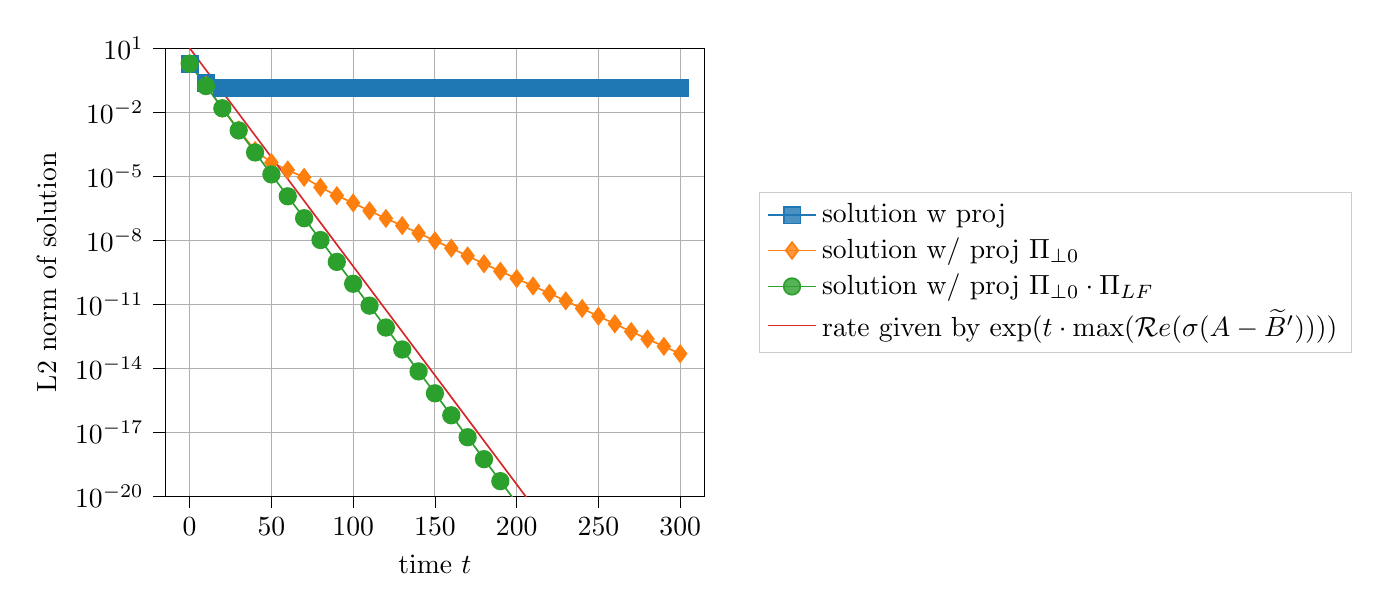
\begin{tikzpicture}

\definecolor{crimson2143940}{RGB}{214,39,40}
\definecolor{darkgray176}{RGB}{176,176,176}
\definecolor{darkorange25512714}{RGB}{255,127,14}
\definecolor{forestgreen4416044}{RGB}{44,160,44}
\definecolor{lightgray204}{RGB}{204,204,204}
\definecolor{steelblue31119180}{RGB}{31,119,180}

\begin{axis}[
legend cell align={left},
legend style={
  fill opacity=0.8,
  draw opacity=1,
  text opacity=1,
  at={(1.1,0.5)},
  anchor=west,
  draw=lightgray204
},
log basis y={10},
tick align=outside,
tick pos=left,
x grid style={darkgray176},
xlabel={time $t$},
xmajorgrids,
xmin=-15, xmax=315,
xtick style={color=black},
y grid style={darkgray176},
ylabel={L2 norm of solution},
ymajorgrids,
ymin=1e-20, ymax=10,
ymode=log,
ytick style={color=black},
ytick={1e-23,1e-20,1e-17,1e-14,1e-11,1e-08,1e-05,0.01,10,10000},
yticklabels={
  $\mathdefault{10^{-23}}$,
  $\mathdefault{10^{-20}}$,
  $\mathdefault{10^{-17}}$,
  $\mathdefault{10^{-14}}$,
  $\mathdefault{10^{-11}}$,
  $\mathdefault{10^{-8}}$,
  $\mathdefault{10^{-5}}$,
  $\mathdefault{10^{-2}}$,
  $\mathdefault{10^{1}}$,
  $\mathdefault{10^{4}}$
}
]
\addplot [semithick, steelblue31119180, mark=square*, mark size=3, mark options={solid}]
table {%
0 1.87090036052962
10 0.225724430417724
20 0.136320441528505
30 0.135412894798565
40 0.135395735021801
50 0.135394298042564
60 0.135394244866486
70 0.135394233585532
80 0.135394232657028
90 0.135394232575127
100 0.135394232580135
110 0.135394232574108
120 0.135394232571477
130 0.13539423256931
140 0.135394232568148
150 0.135394232568053
160 0.135394232568009
170 0.135394232567946
180 0.135394232567922
190 0.135394232567921
200 0.135394232567919
210 0.135394232567917
220 0.135394232567917
230 0.135394232567917
240 0.135394232567917
250 0.135394232567917
260 0.135394232567917
270 0.135394232567917
280 0.135394232567917
290 0.135394232567917
300 0.135394232567917
};
\addlegendentry{solution w\ proj}
\addplot [semithick, darkorange25512714, mark=diamond*, mark size=3, mark options={solid}]
table {%
0 1.87090036052962
10 0.179784385377465
20 0.0152082899497773
30 0.00146742449455237
40 0.000163025955338489
50 4.3859752250752e-05
60 1.97318020564726e-05
70 8.90322380717846e-06
80 3.04408036615443e-06
90 1.24128770464238e-06
100 5.62056622741371e-07
110 2.39610617475715e-07
120 1.05714791135703e-07
130 4.87326670956824e-08
140 2.14781703926709e-08
150 9.57293315697364e-09
160 4.29526116469493e-09
170 1.85018658710645e-09
180 7.96144003705684e-10
190 3.56328909383631e-10
200 1.61030384148974e-10
210 7.22470651823345e-11
220 3.26176790491538e-11
230 1.45831173914201e-11
240 6.39852604150518e-12
250 2.78615110956797e-12
260 1.21260613717765e-12
270 5.30966957688483e-13
280 2.36728944555156e-13
290 1.07218340679466e-13
300 4.86541565843685e-14
};
\addlegendentry{solution w/ proj $\Pi_{\perp 0}$}
\addplot [semithick, forestgreen4416044, mark=*, mark size=3, mark options={solid}]
table {%
0 1.87090036052962
10 0.167906622547116
20 0.0152547158371657
30 0.00140243380228884
40 0.000130271657311899
50 1.21996641201202e-05
60 1.14899386812342e-06
70 1.08585155527167e-07
80 1.02774382718609e-08
90 9.72839436261965e-10
100 9.20053398256894e-11
110 8.68841191975079e-12
120 8.19025657310313e-13
130 7.70661542908942e-14
140 7.23934557421525e-15
150 6.79088664589721e-16
160 6.36375010784999e-17
170 5.96016805754538e-18
180 5.58185862152816e-19
190 5.22987905372147e-20
200 4.90454962230999e-21
210 4.60543985832032e-22
220 4.33141290181463e-23
230 4.08072338606358e-24
240 3.85116042992489e-25
250 3.64022180393027e-26
260 3.44530068265139e-27
270 3.26386468804083e-28
280 3.0936090087328e-29
290 2.93257059974141e-30
300 2.77919717615354e-31
};
\addlegendentry{solution w/ proj $\Pi_{\perp 0}\cdot\Pi_{LF}$}
\addplot [semithick, crimson2143940]
table {%
0 10
10 0.951111830888997
20 0.090461371485702
30 0.00860388806584957
40 0.000818325973107418
50 7.78319514546217e-05
60 7.40268898496687e-06
70 7.04078507399366e-07
80 6.69657398262203e-08
90 6.36919074129526e-09
100 6.05781266723458e-10
110 5.76165729711604e-11
120 5.47998042081499e-12
130 5.2120742112772e-13
140 4.95726544581719e-14
150 4.71491381437395e-15
160 4.48441031047303e-16
170 4.2651757008515e-17
180 4.05665906990013e-18
190 3.85833643526517e-19
200 3.66970943113078e-20
210 3.49030405587341e-21
220 3.31966948094105e-22
230 3.15737691796417e-23
240 3.00301854125156e-24
250 2.85620646296337e-25
260 2.71657175838608e-26
270 2.58376353885993e-27
280 2.45744807002931e-28
290 2.3373079332002e-29
300 2.22304122769743e-30
};
\addlegendentry{rate given by $\exp(t\cdot\max(\mathcal{R}e(\sigma(A-\widetilde{B}'))))$}
\end{axis}

\end{tikzpicture}
